\documentclass{uc3mpracticas}

\usepackage{helvet}
\usepackage{caption}
\usepackage{listings}
\renewcommand{\familydefault}{\sfdefault}


%%%%%%%%%%%%%%%%%%%%%%%%%%%%%%%%%%%%%%%%%%%%%%%%%%%%%%%%%%%%%%%%%%%%%%%%%%%%%%%%
%%%                   Plantilla Prácticas UC3M                               %%%
%%%                Universidad Carlos III de Madrid                          %%%
%%%                   Alejandro Valverde Mahou                               %%%
%%%%%%%%%%%%%%%%%%%%%%%%%%%%%%%%%%%%%%%%%%%%%%%%%%%%%%%%%%%%%%%%%%%%%%%%%%%%%%%%

%Permitir cabeceras y pie de páginas personalizados
\pagestyle{fancy}

%Path por defecto de las imágenes
\graphicspath{ {./images/} }

%Declarar formato de encabezado y pie de página de las páginas del documento
\fancypagestyle{doc}{
  %Cabecera
  \headerpr[1]{Planificación Automática}{}{Ingeniería del Conocimiento}
  %Pie de Página
  \footerpr{}{\textbf{UC3M}}{{\thepage} de \pageref{LastPage}}
}

%Declarar formato de encabezado y pie del título e indice
\fancypagestyle{titu}{%
  %Cabecera
  \headerpr{}{}{}
  %Pie de Página
  \footerpr{}{}{}
}


\appto\frontmatter{\pagestyle{titu}}
\appto\mainmatter{\pagestyle{doc}}


\begin{document}
  %Comienzo formato título
  \frontmatter


  %Portada 1 (Centrado todo)
  \centeredtitle{Images/LogoUC3M.png}{Grado en Ingeniería Informática}{Curso 2020/2021}{Ingeniería del Conocimiento}{Práctica 2: Planificación Automática}

  \vspace{55mm}

  \authors{Alba Reinders Sánchez}{100383444}{Alejandro Valverde Mahou}{100383383}{}{}{Grupo 83}{Leganés}

  \newpage

  %Índice
  \tableofcontents

  \newpage

  %Comienzo formato documento general
  \mainmatter

  \section{Introducción}

  En esta segunda práctica se lleva a cabo el modelado de un problema similar al de la práctica anterior pero en este caso un \textbf{planificador} tiene que que simular una sesión entre el robot y el paciente, donde la actividad que realizan es jugar al \textbf{juego de memoria de las cartas}.

  \vspace{2mm}

  El documento consiste en el manual técnico con la descripción del dominio implementado, el manual de usuario con la explicación de cómo usar el programa, las pruebas realizadas y el análisis de los resultados, y para finalizar una serie de conclusiones y comentarios personales.

  \section{Manual técnico}

  A continuación se describe el dominio creado explicando los \textit{predicados} y las \textit{acciones}, en cada acción se especifican sus precondiciones y efectos. Además, se justifican todas las decisiones que se han tenido que tomar durante la implementación.

  \vspace{2mm}

  El flujo de una sesión que se ha planteado es el que se muestra en el siguiente diagrama de estados, donde se pueden ver todas las acciones implementadas para el correcto funcionamiento del planificador.


  \begin{figure}[!h]
    \centering
    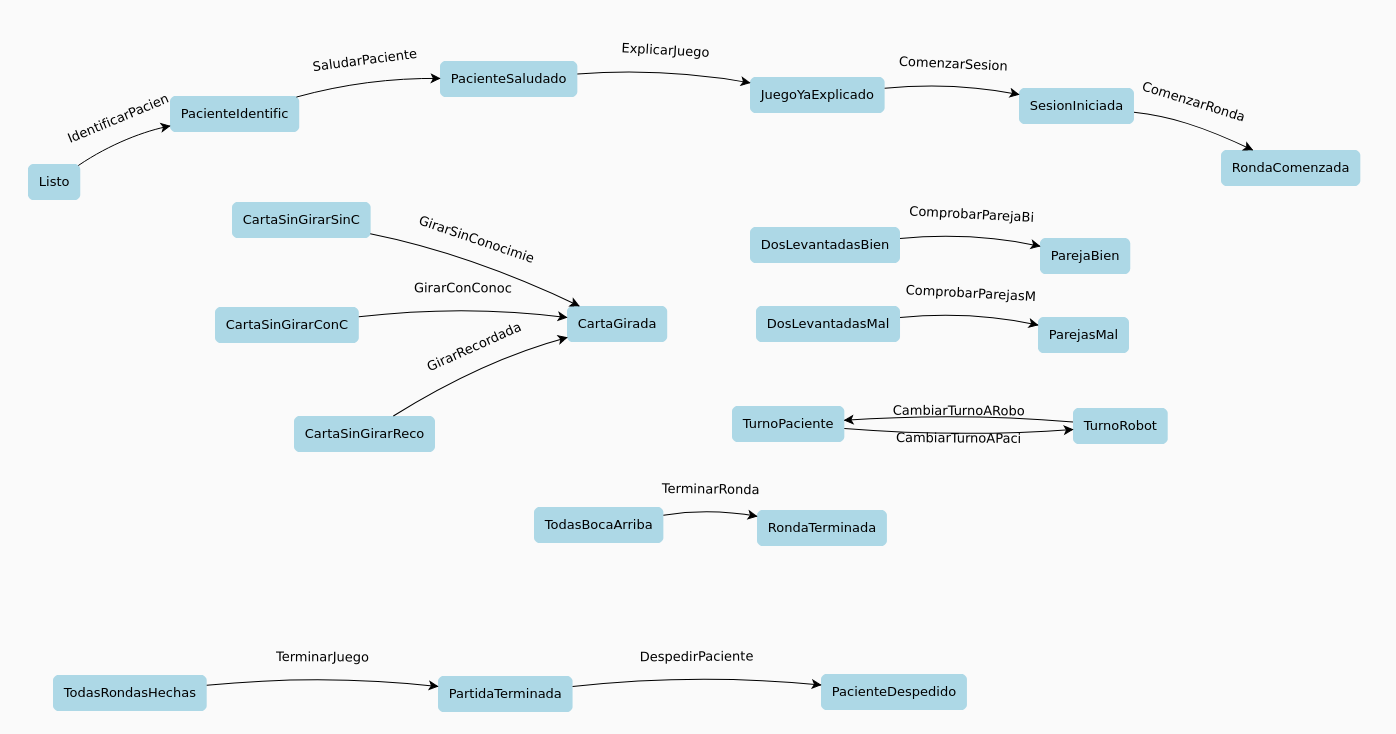
\includegraphics[width=1.1\linewidth]{./Images/flujo.png}
    \caption*{Flujo de una sesión}
  \end{figure}



  \subsection{Predicados}

  Los predicados que se crean para el dominio son los siguientes:

  \begin{itemize}
    \item \textbf{Existe Paciente ?p}: indica el nombre del paciente que va a recibir la sesión.
    \item \textbf{Identificado ?idp}: indica que el paciente ha sido identificado por el robot.
    \item \textbf{Saludado ?sp}: indica que el paciente ha sido saludado por el robot.
    \item \textbf{JuegoExplicado ?jp}: indica que se le ha explicado el juego al paciente.
    \item \textbf{RondaInicial ?r}: indica el nombre de la ronda inicial.
    \item \textbf{RondaActual ?r}: indica el nombre de la ronda actual de la sesión.
    \item \textbf{Siguiente ?r1 ?r2}: indica el orden de las rondas, se pasa de \textit{?r1} a \textit{?r2}.
    \item \textbf{Turno ?t}: indica de quién es el turno.
    \item \textbf{CartaEnRonda ?c ?r}: indica en qué ronda se va a usar cada carta.
    \item \textbf{ParejaCartas ?c1 ?c2}: indica que dos cartas forman una pareja.
    \item \textbf{CartaBocaArriba ?c}: indica que una  carta se encuentra boca arriba.
    \item \textbf{CartaRecordada ?c}: indica que una carta ya ha sido dada la vuelta y es recordada por los jugadores.
    \item \textbf{CartaEmparejada ?c}: indica que una carta ya ha sido emparejada correctamente.
    \item \textbf{JuegoTerminado}: indica que el juego ha acabado.
    \item \textbf{Despedido ?dp}: indica que el paciente ha sido despedido por el robot.
  \end{itemize}

  \subsection{Funciones}

  \begin{itemize}
    \item \textbf{Contador Boca Arriba}: indica el número de cartas dadas la vuelta y sirve para determinar cuando hay que realizar las comprobaciones.
  \end{itemize}


  Hemos puesto carta en ronda pero la roinda actual es variable y hay que cambiarlo. Para ello hay que hacer otro predicado que sea next que indique el orden de las rondas. (como en el simon)


  \subsection{Acciones}

  Respecto a las acciones, se han elaborado todas las necesarias para poder realizar una sesión normal, acciones comunes para ambos jugadores y acciones exclusivas del robot. También se tiene en cuenta que la sesión puede ser interrumpida y para ello se crea una acción especial (X).

  \vspace{2mm}

  Por lo que se van a explicar cada una de las acciones del dominio junto con sus precondiciones y efectos para que sea más clara la explicación.

  \begin{itemize}
    \item \textbf{Identificar Paciente}: acción del robot que permite pasar del estado inicial al momento en el que se ha reconocido al paciente.

      \textit{Precondiciones}: que exista un paciente, y que no haya sido identificado todavía.

      \textit{Efectos}: el paciente pasa a estar identificado.

    \item \textbf{Saludar Paciente}: acción del robot por la que se saluda a un paciente que ya ha sido identificado, antes de empezar un juego.

      \textit{Precondiciones}: que exista un paciente que haya sido identificado, pero no saludado.

      \textit{Efectos}: saludar al paciente

    \item \textbf{Explicar Juego}: acción del robot en la que este explica las reglas del juego de las cartas.

      \textit{Precondiciones}: que exista un paciente que haya saludado, pero que no se le haya explicado el juego.

      \textit{Efectos}: se le explica el juego al paciente.

    \item \textbf{Comenzar Sesión}: acción del robot que da comienzo al juego.

      \textit{Precondiciones}: que haya un paciente al que se le haya explicado el juego y que exista una ronda inicial.

      \textit{Efectos}: se establece como ronda actual la ronda inicial.

    \item \textbf{Comenzar Ronda}: acción del robot que da comienzo a una nueva ronda.

      \textit{Precondiciones}: que se haya preparado una ronda.

      \textit{Efectos}: es el turno del paciente.

    \item \textbf{Girar Sin Conocimiento}: acción del robot o del paciente en la que se gira una carta de forma aleatoria porque no se tiene ningún conocimiento previo.

      \textit{Precondiciones}: que se haya iniciado una ronda, que el contador de cartas boca arriba sea 0 o 1, que no haya conocimiento sobre ninguna carta y que la carta esté boca abajo.

      \textit{Efectos}: la carta pasa a estar boca arriba, aumenta el número de cartas boca arriba y la carta pasa a ser recordada por los jugadores.

    \item \textbf{Girar Con Conocimiento}: acción del robot o del paciente en la que se gira una carta conociendo la posición de alguna otra.

      \textit{Precondiciones}: que se haya iniciado una ronda, que el contador de cartas boca arriba sea 0 o 1, que haya conocimiento sobre alguna carta y que la carta esté boca abajo.

      \textit{Efectos}: la carta pasa a estar boca arriba, aumenta el número de cartas boca arriba y la carta pasa a ser recordada por los jugadores.

    \item \textbf{Girar Recordada}: acción del robot o del paciente en la que se gira una carta conociendo la carta previamente.

      \textit{Precondiciones}: que se haya iniciado una ronda, que el contador de cartas boca arriba sea 0 o 1, que haya conocimiento sobre la carta que se va a girar y que esté boca abajo.

      \textit{Efectos}: la carta pasa a estar boca arriba y aumenta el número de cartas boca arriba.

    \item \textbf{Comprobar Pareja Bien}: acción del robot por la que se comprueba que una pareja de cartas boca arriba sea correcta.

      \textit{Precondiciones}: que haya dos carta boca arriba, que no estén emparejadas correctamente y que ambas formen una pareja.

      \textit{Efectos}: se resetea el contador de cartas boca arriba y las cartas pasan a estar emparejadas correctamente.

    \item \textbf{Comprobar Pareja Mal}: acción del robot por la que se comprueba que una pareja de cartas boca arriba no sea correcta.

      \textit{Precondiciones}: que haya dos carta boca arriba, que no estén emparejadas correctamente y que ambas no formen una pareja.

      \textit{Efectos}: se resetea el contador de cartas boca arriba y las cartas pasan a estar boca abajo.

    \item \textbf{Cambiar Turno A Robot}: acción del robot por la que se cambia de turno una vez haya dos cartas boca arriba.

      \textit{Precondiciones}: que el contador de cartas boca arriba se haya reseteado, que sea el turno del paciente y que siga habiendo cartas boca abajo.

      \textit{Efectos}: pasa a ser el turno del robot y el contador de cartas boca arriba se pone a 0.

    \item \textbf{Cambiar Turno A Paciente}: acción del robot por la que se cambia de turno una vez haya dos cartas boca arriba.

      \textit{Precondiciones}: que el contador de cartas boca arriba se haya reseteado, que sea el turno del robot y que siga habiendo cartas boca abajo.

      \textit{Efectos}: pasa a ser el turno del paciente y el contador de cartas boca arriba se pone a 0.

    \item \textbf{Terminar Ronda}: acción del robot por la que se termina la ronda actual.

      \textit{Precondiciones}: que el contador de cartas boca arriba se haya reseteado y que no haya cartas de la ronda boca abajo.

      \textit{Efectos}: pasa a ser el turno del paciente, el contador de cartas boca arriba se pone a 0 y el contandor de rondas aumenta.

    \item \textbf{Terminar Juego}: acción del robot que termina la sesión una vez se han realizado las rondas establecidas.

      \textit{Precondiciones}: que el contador de rondas actuales sea igual al total de rondas.

      \textit{Efectos}: terminar la sesión.

    \item \textbf{Despedir Paciente}: acción del robot que despide al paciente una vez se ha terminado la sesión.

      \textit{Precondiciones}: que la sesión se haya terminado.

      \textit{Efectos}: despedirse del paciente.


  \end{itemize}









  \section{Manual de usuario}


  \section{Pruebas realizadas}


  \section{Conclusiones}


  \section{Comentarios personales}




\end{document}
